\documentclass[12pt]{article}
 
\usepackage[margin=1in]{geometry}
\usepackage{amsmath,amsthm,amssymb}
\usepackage{listings}
\usepackage{graphicx}
\graphicspath{ {figures/} }
\usepackage{booktabs}
\usepackage{listings}
\usepackage{float}
\usepackage{subcaption}

\newcommand{\N}{\mathbb{N}}
\newcommand{\R}{\mathbb{R}}
\newcommand{\Z}{\mathbb{Z}}
\newcommand{\Q}{\mathbb{Q}}
 
\newenvironment{theorem}[2][Theorem]{\begin{trivlist}
\item[\hskip \labelsep {\bfseries #1}\hskip \labelsep {\bfseries #2.}]}{\end{trivlist}}
\newenvironment{lemma}[2][Lemma]{\begin{trivlist}
\item[\hskip \labelsep {\bfseries #1}\hskip \labelsep {\bfseries #2.}]}{\end{trivlist}}
\newenvironment{exercise}[2][Exercise]{\begin{trivlist}
\item[\hskip \labelsep {\bfseries #1}\hskip \labelsep {\bfseries #2.}]}{\end{trivlist}}
\newenvironment{problem}[2][Problem]{\begin{trivlist}
\item[\hskip \labelsep {\bfseries #1}\hskip \labelsep {\bfseries #2.}]}{\end{trivlist}}
\newenvironment{question}[2][Question]{\begin{trivlist}
\item[\hskip \labelsep {\bfseries #1}\hskip \labelsep {\bfseries #2.}]}{\end{trivlist}}
\newenvironment{corollary}[2][Corollary]{\begin{trivlist}
\item[\hskip \labelsep {\bfseries #1}\hskip \labelsep {\bfseries #2.}]}{\end{trivlist}}
 
\begin{document}
 
\title{Homework 2}
\author{Ningyu Ma\\ 
ME614 Spring 2017}

\maketitle
\begin{problem}{1}
\text{}\\
$(a)$ For $n_{max}$, I find it in python using the command,
\begin{lstlisting}[language=Python]
while np.isfinite(pi_star * np.pi)
\end{lstlisting}
where $\hat{\pi}^{*}$ and $\pi$ are in float16, float32 and float64 format respectively.
I find that the $n_{max}$ for float16, float32 and float64 are 7, 76, 619 respectively.\\
\\
From Figure 1 to 3, we can see that the round off error increase with bigger $n$ and it is larger for less precise format and smaller for better precise format.\\
\begin{figure}[H]
\centering
  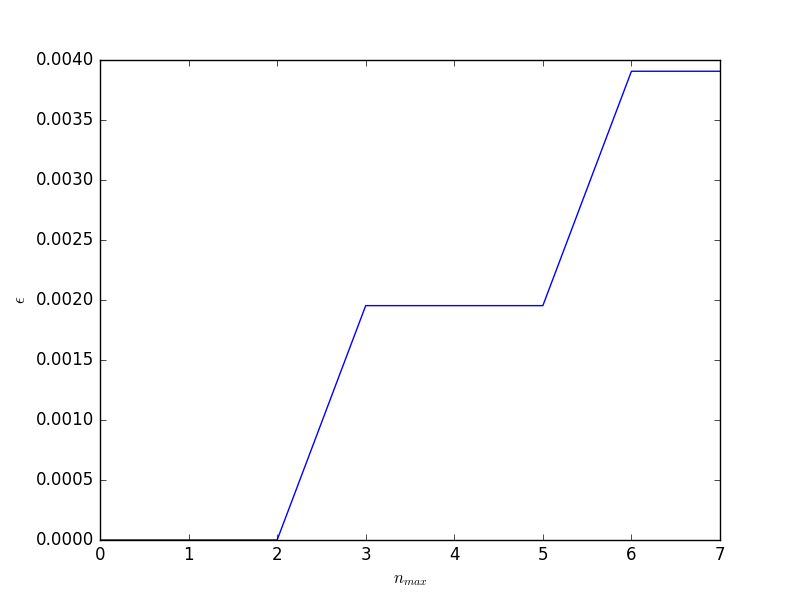
\includegraphics[scale=0.65]{p1_f16.png}
 \caption{Round off Error $\epsilon$ vs. $n$ for float16}
\label{label}
\end{figure}
\begin{figure}[H]
\centering
  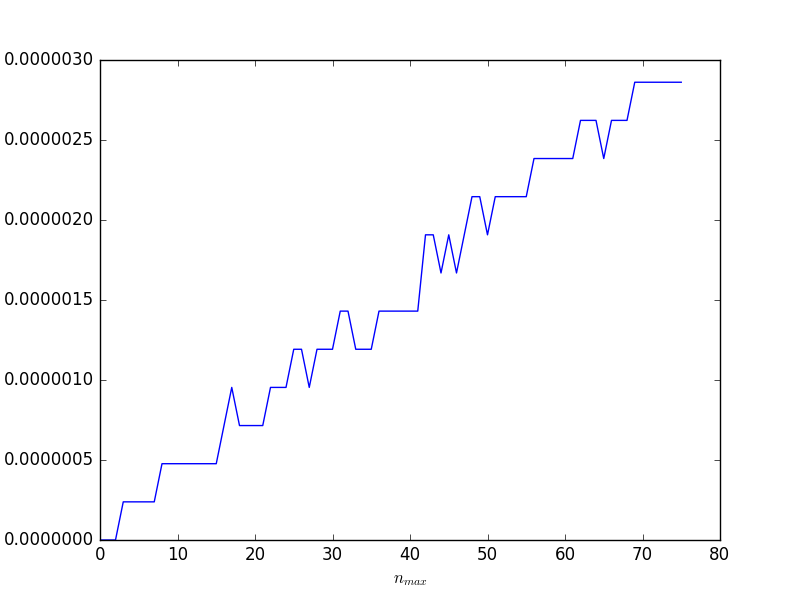
\includegraphics[scale=0.65]{p1_f32.png}
 \caption{Round off Error $\epsilon$ vs. $n$ for float32}
\label{label}
\end{figure}
\begin{figure}[H]
\centering
  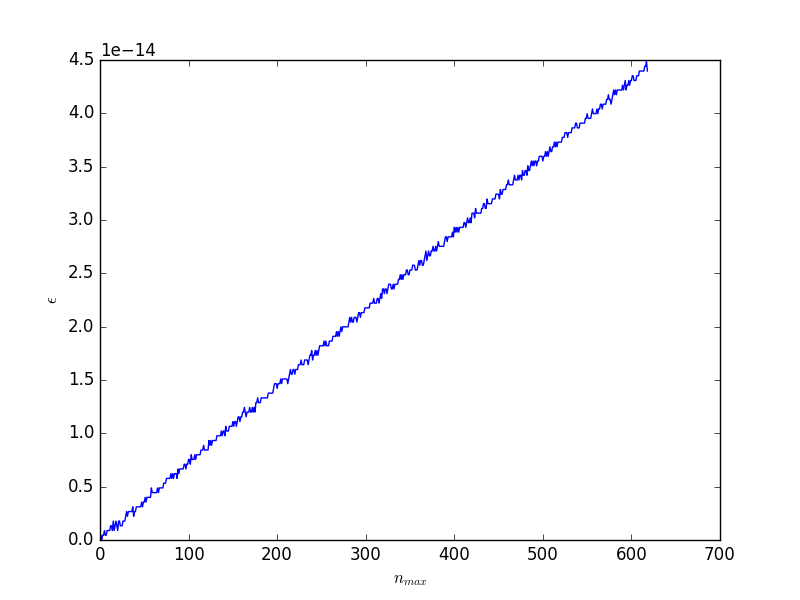
\includegraphics[scale=0.65]{p1_f64.png}
 \caption{Round off Error $\epsilon$ vs. $n$ for float64}
\label{label}
\end{figure}
\end{problem}

\begin{problem}{2}
\text{}\\
$(a)$ for $u(x,t) = c_{1}e^{(-\omega_1^{2} \alpha t)}sin(\omega_{1}(x-ct)-\gamma_{1}) - c_{2}e^{(-\omega_2^{2} \alpha t)}cos(\omega_{2}(x-ct)-\gamma_{2})$, if we plug it in to the advection/diffusion equation, we can get:\\
\\
$\frac{\partial u}{\partial t} =  c_{1}(-\omega_{1}^2 \alpha)e^{(-\omega_1^{2} \alpha t)}sin(\omega_{1}(x-ct)-\gamma_{1}) + c_{1}(-\omega_1 c)e^{(-\omega_1^{2} \alpha t)}cos(\omega_{1}(x-ct)-\gamma_{1}) -\\c_{2}(-\omega_{2}^2 \alpha)e^{(-\omega_2^{2} \alpha t)}cos(\omega_{2}(x-ct)-\gamma_{2}) + + c_{2}(-\omega_2 c)e^{(-\omega_2^{2} \alpha t)}sin(\omega_{2}(x-ct)-\gamma_{2})$\\
\\
$\frac{\partial u}{\partial x} =  c_{1} \omega_{1}e^{(-\omega_1^{2} \alpha t)}cos(\omega_{1}(x-ct)-\gamma_{1}) + c_{2} \omega_{2}e^{(-\omega_2^{2} \alpha t)}sin(\omega_{2}(x-ct)-\gamma_{2})$\\
\\
$\frac{\partial^2 u}{\partial x^2} =  -c_{1} \omega_{1}^2 e^{(-\omega_1^{2} \alpha t)}sin(\omega_{1}(x-ct)-\gamma_{1}) + c_{2} \omega_{2}^2 e^{(-\omega_2^{2} \alpha t)}cos(\omega_{2}(x-ct)-\gamma_{2})$\\
\\
And we can see that $\frac{\partial u}{\partial t} + c \frac{\partial u}{\partial x} - \alpha \frac{\partial^2 u}{\partial x^2} = 0$\\
\text{}\\
$(b)$ Figure 4 to 7, we can see the results from python code.  We can see that the results are indistinguishable between each scheme combination when $N$ is large.\\
So I calculated the root-square-mean for each scheme combination w.r.t. the Analytical solution.\\
From the result of python code, the best scheme is 2nd-order-central \& Crank-Nicolson for all four cases and least performing one is 1st-order-upwind \& Explicit-Euler scheme.\\
\begin{figure}[H]
\centering
  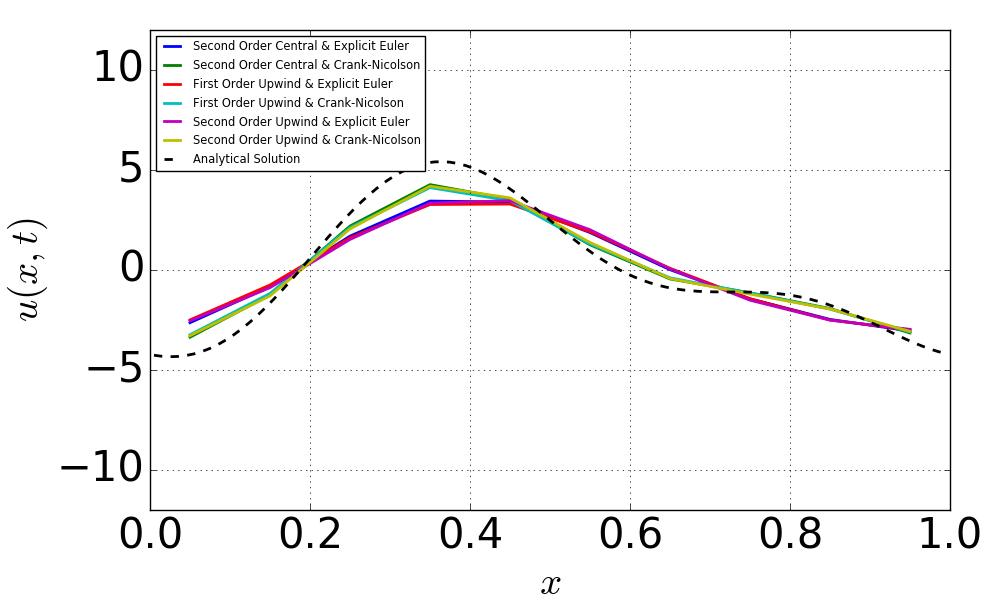
\includegraphics[scale=0.65]{p2b_n10.png}
 \caption{Numerical Solution at $t=t_f$ with $N=10$}
\label{label}
\end{figure}
\begin{figure}[H]
\centering
  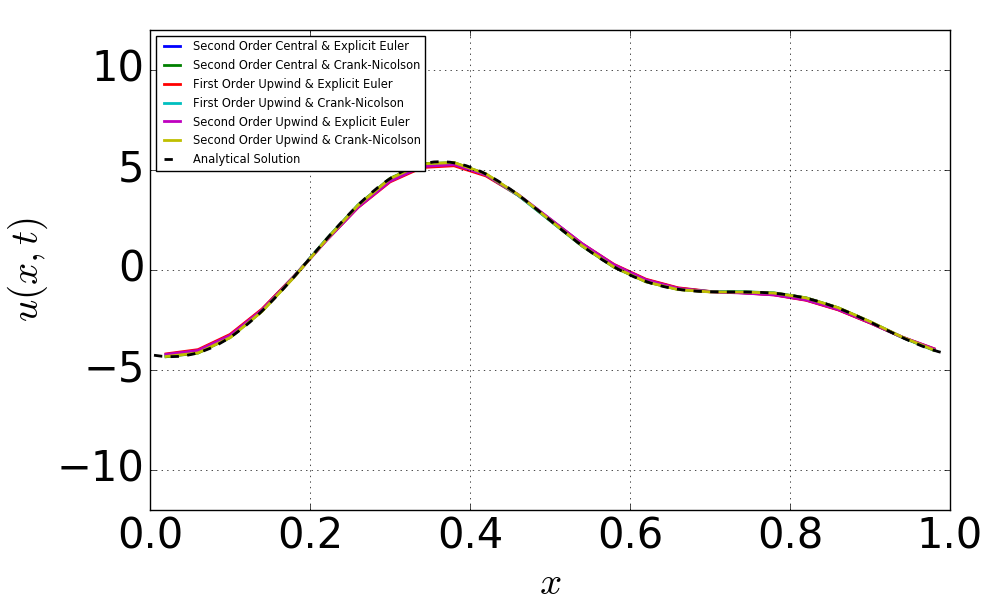
\includegraphics[scale=0.65]{p2b_n25.png}
 \caption{Numerical Solution at $t=t_f$ with $N=25$}
\label{label}
\end{figure}
\begin{figure}[H]
\centering
  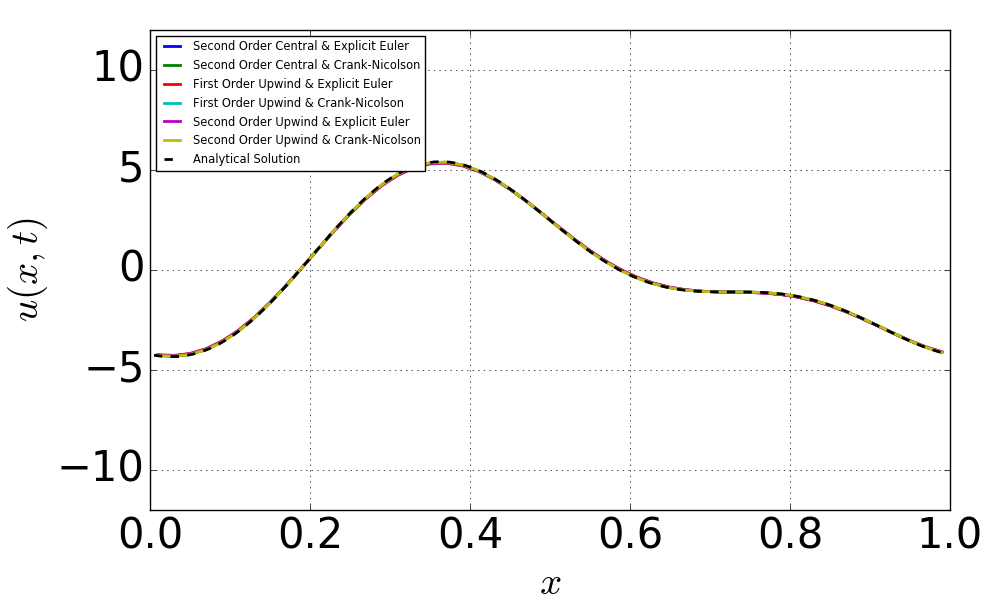
\includegraphics[scale=0.65]{p2b_n50.png}
 \caption{Numerical Solution at $t=t_f$ with $N=50$}
\label{label}
\end{figure}
\begin{figure}[H]
\centering
  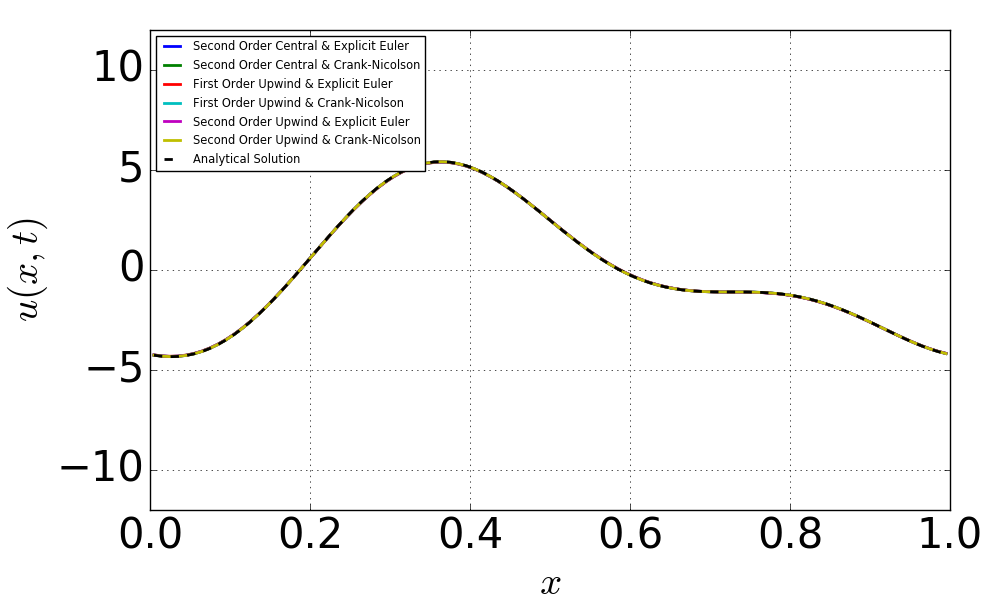
\includegraphics[scale=0.65]{p2b_n100.png}
 \caption{Numerical Solution at $t=t_f$ with $N=100$}
\label{label}
\end{figure}
\text{}\\
$(c)$ \\
From Figure 8, which is the case of fixed small $\Delta t$ with changing $\Delta x$, we can see that for the two second order spatial discretization scheme, the order of accuracy is second order, and for the one first order upwind scheme, the order of accuracy is one.\\
\begin{figure}[H]
\centering
  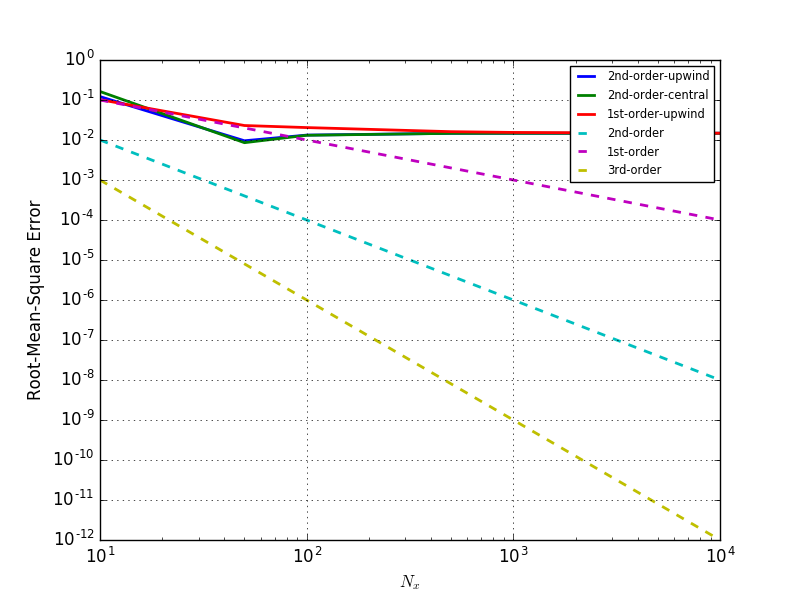
\includegraphics[scale=0.65]{p2c_fixed_dt.png}
 \caption{Root-Mean-Square Error at $t=T_f$ vs. Number of Points $N$}
\label{label}
\end{figure}
From Figure 9, which is the case of fixed small $\Delta x$ with changing $\Delta t$, we can see that for the for all of those three schemes, the order of accuracy are all second order approximately. Because the order of accuracy of Crank-Nicolson is two. \\
\begin{figure}[H]
\centering
  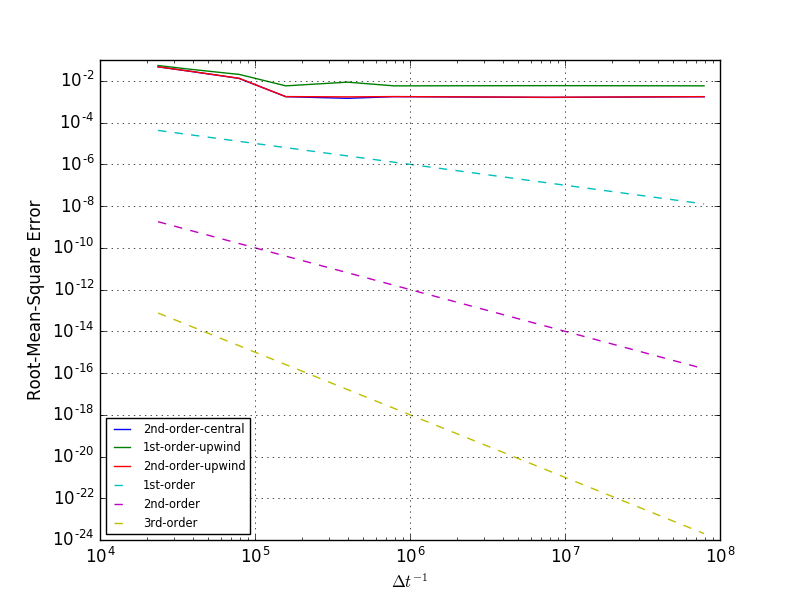
\includegraphics[scale=0.65]{p2c_fixed_dx.png}
 \caption{Root-Mean-Square Error at $t=T_f$ vs. $\delta t$}
\label{label}
\end{figure}
\text{}\\
$(d)$ Please see Figure 10 to 15 for the spy of $\mathbf{A}$ and $\mathbf{B}$.\\
\begin{figure}[H]
\centering
  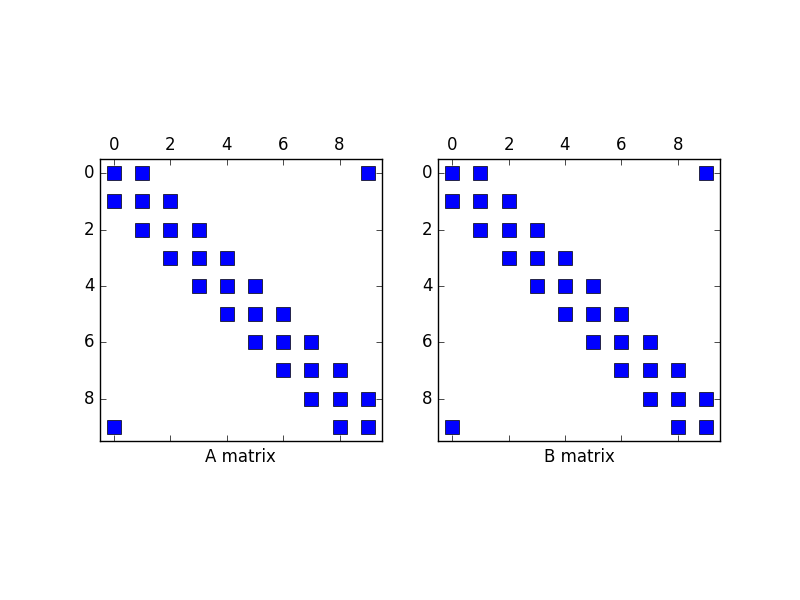
\includegraphics[scale=0.5]{p2d_1st_cn.png}
 \caption{Spy Plot of $\mathbf{A}$ and $\mathbf{B}$ for 1st-order-upwind \& Crank-Nicolson}
\label{label}
\end{figure}
\begin{figure}[H]
\centering
  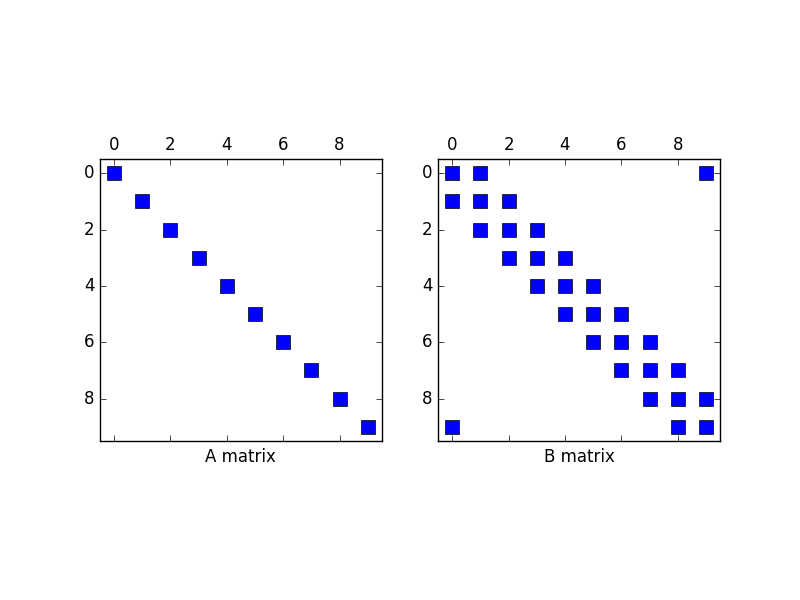
\includegraphics[scale=0.5]{p2d_u1st_ee.png}
 \caption{Spy Plot of $\mathbf{A}$ and $\mathbf{B}$ for 1st-order-upwind \& Explicit-Euler}
\label{label}
\end{figure}
\begin{figure}[H]
\centering
  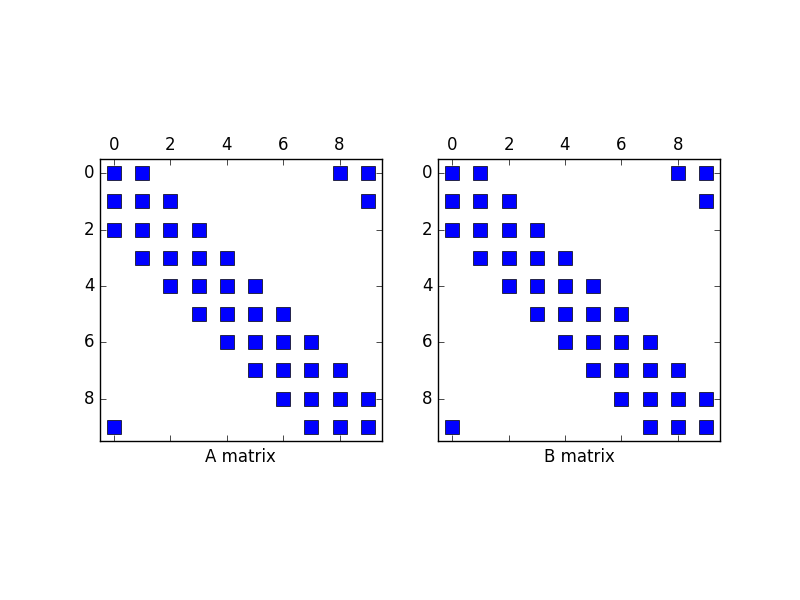
\includegraphics[scale=0.5]{p2d_u2nd_cn.png}
 \caption{Spy Plot of $\mathbf{A}$ and $\mathbf{B}$ for 2nd-order-upwind \& Crank-Nicolson}
\label{label}
\end{figure}
\begin{figure}[H]
\centering
  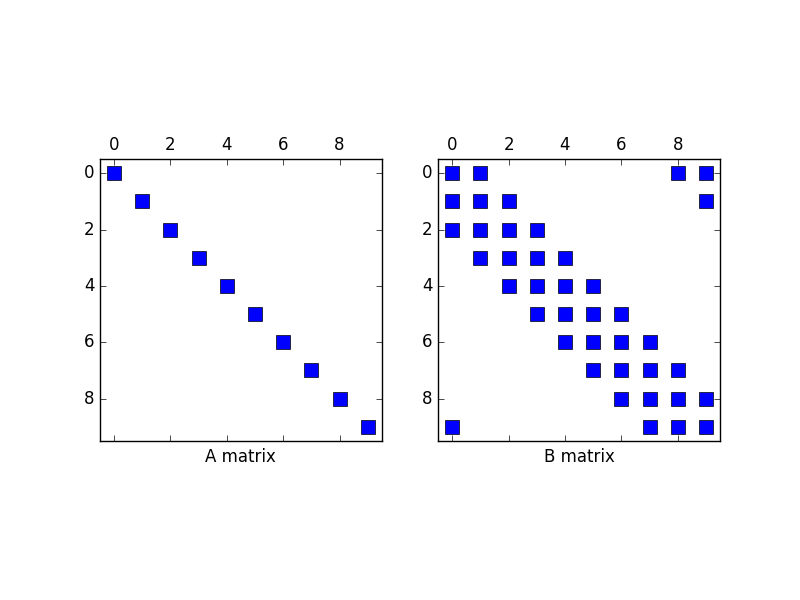
\includegraphics[scale=0.5]{p2d_u2nd_ee.png}
 \caption{Spy Plot of $\mathbf{A}$ and $\mathbf{B}$ for 2nd-order-upwind \& Explicit-Euler}
\label{label}
\end{figure}
\begin{figure}[H]
\centering
  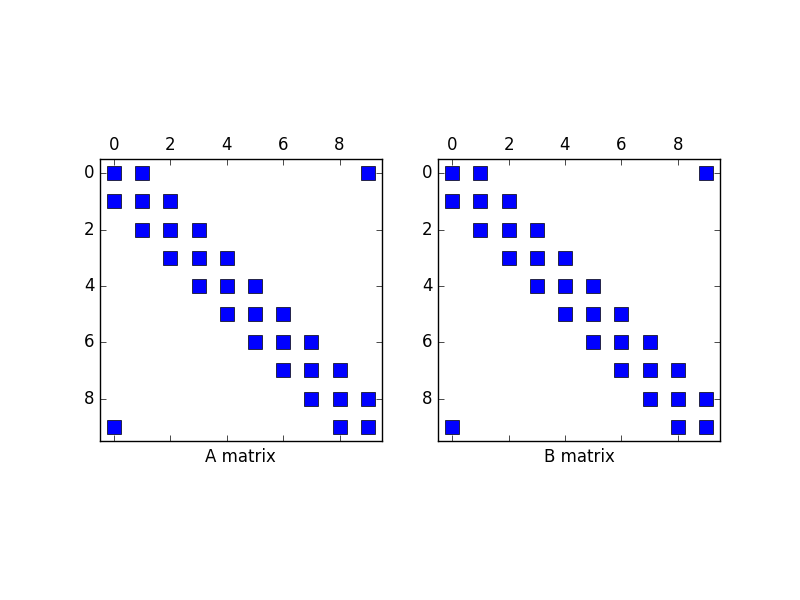
\includegraphics[scale=0.5]{p2d_c2nd_cn.png}
 \caption{Spy Plot of $\mathbf{A}$ and $\mathbf{B}$ for 2nd-order-central \& Crank-Nicolson}
\label{label}
\end{figure}
\begin{figure}[H]
\centering
  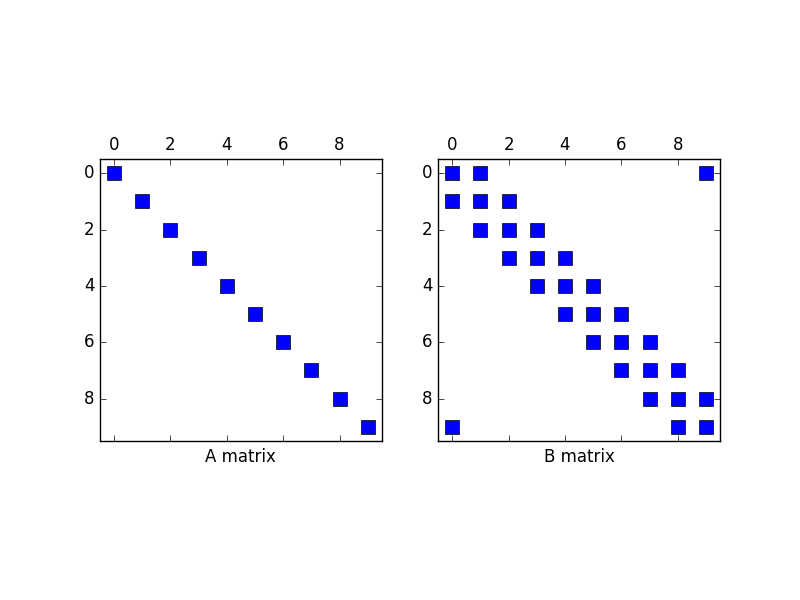
\includegraphics[scale=0.5]{p2d_c2nd_ee.png}
 \caption{Spy Plot of $\mathbf{A}$ and $\mathbf{B}$ for 2nd-order-central \& Explicit-Euler}
\label{label}
\end{figure}
\text{}\\
$(e)$
From Figure 16 to 18, we can see from the contour plots that the green region is the stable region, In green region, for Explicit Euler, the maximum $\lambda$ is exactly 1 with all the other $\lambda$ s below 1. And 2nd-order-central scheme has the largest stable region.\\
\begin{figure}[H]
\centering
  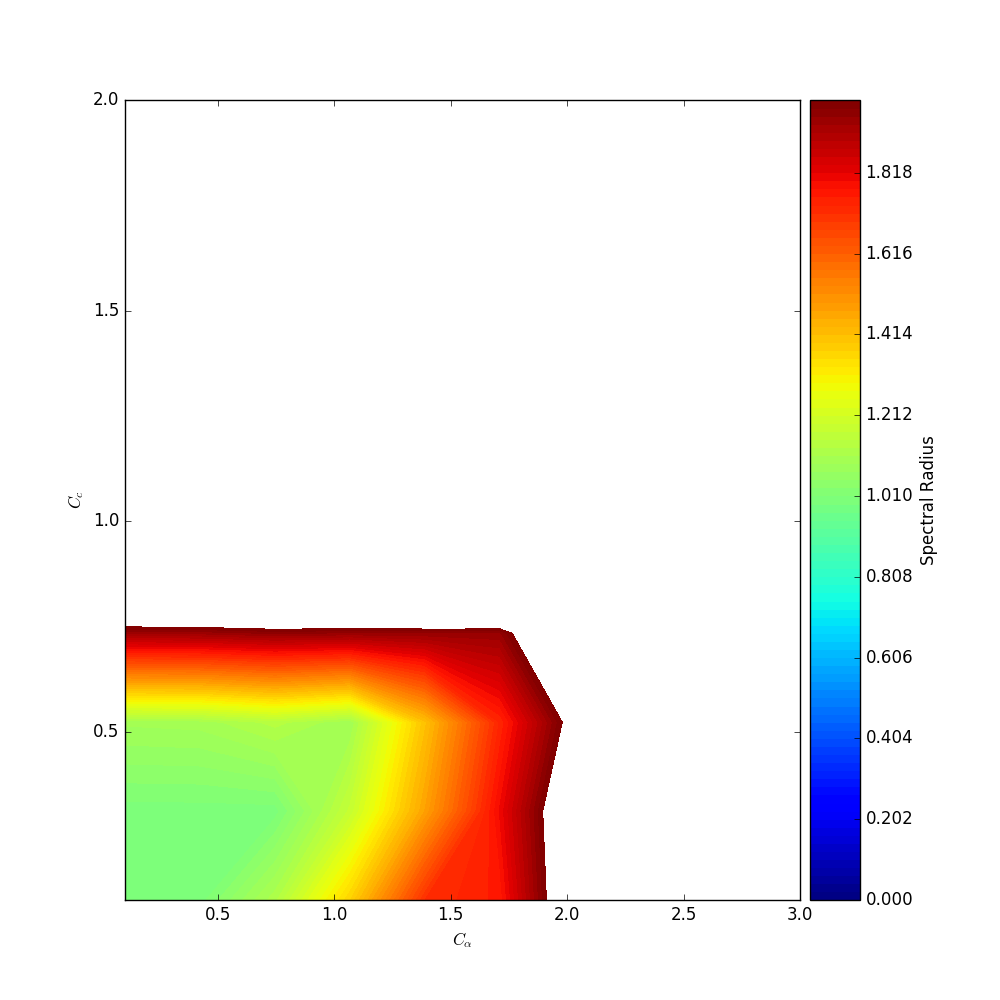
\includegraphics[scale=0.35]{p2e_contours_c2nd.png}
 \caption{Flooded Iso-contour of Spectral Radius for 2nd-order-central}
\label{label}
\end{figure}
\begin{figure}[H]
\centering
  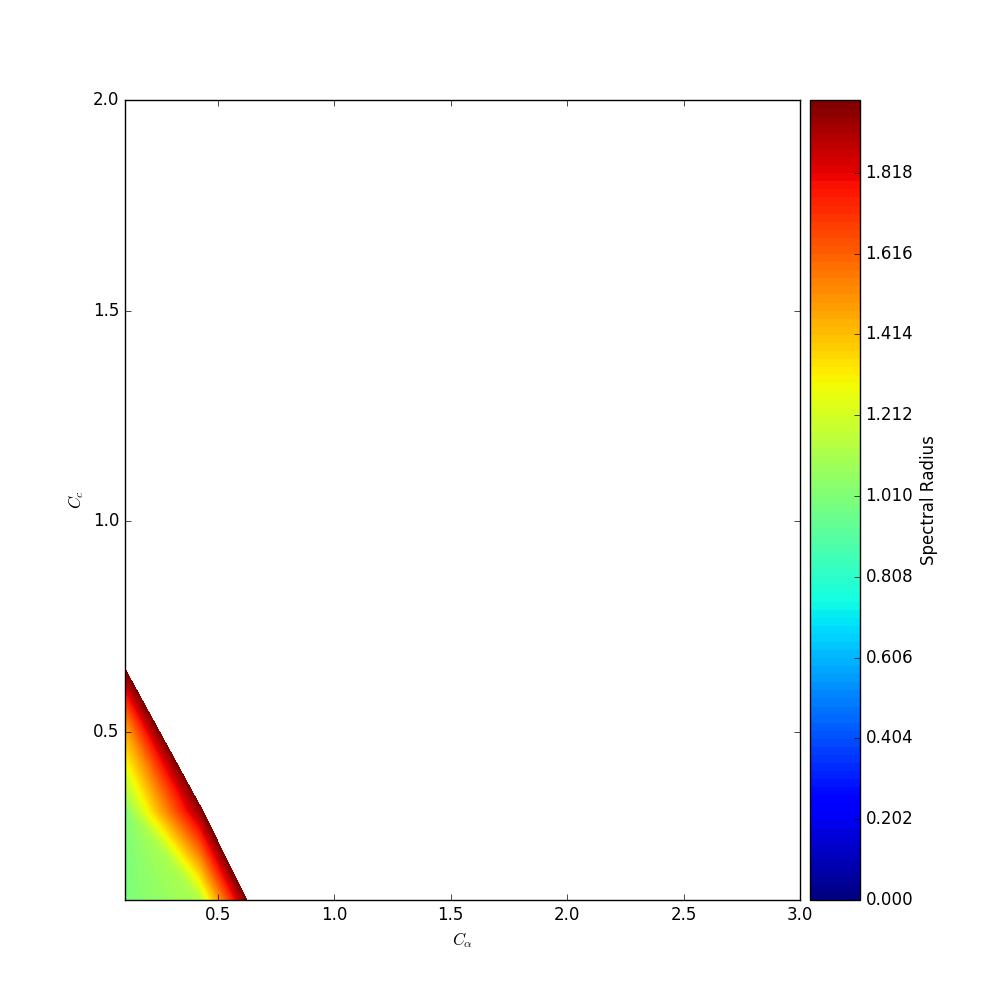
\includegraphics[scale=0.35]{p2e_contours_u2nd.png}
 \caption{Flooded Iso-contour of Spectral Radius for 2nd-order-upwind}
\label{label}
\end{figure}
\begin{figure}[H]
\centering
  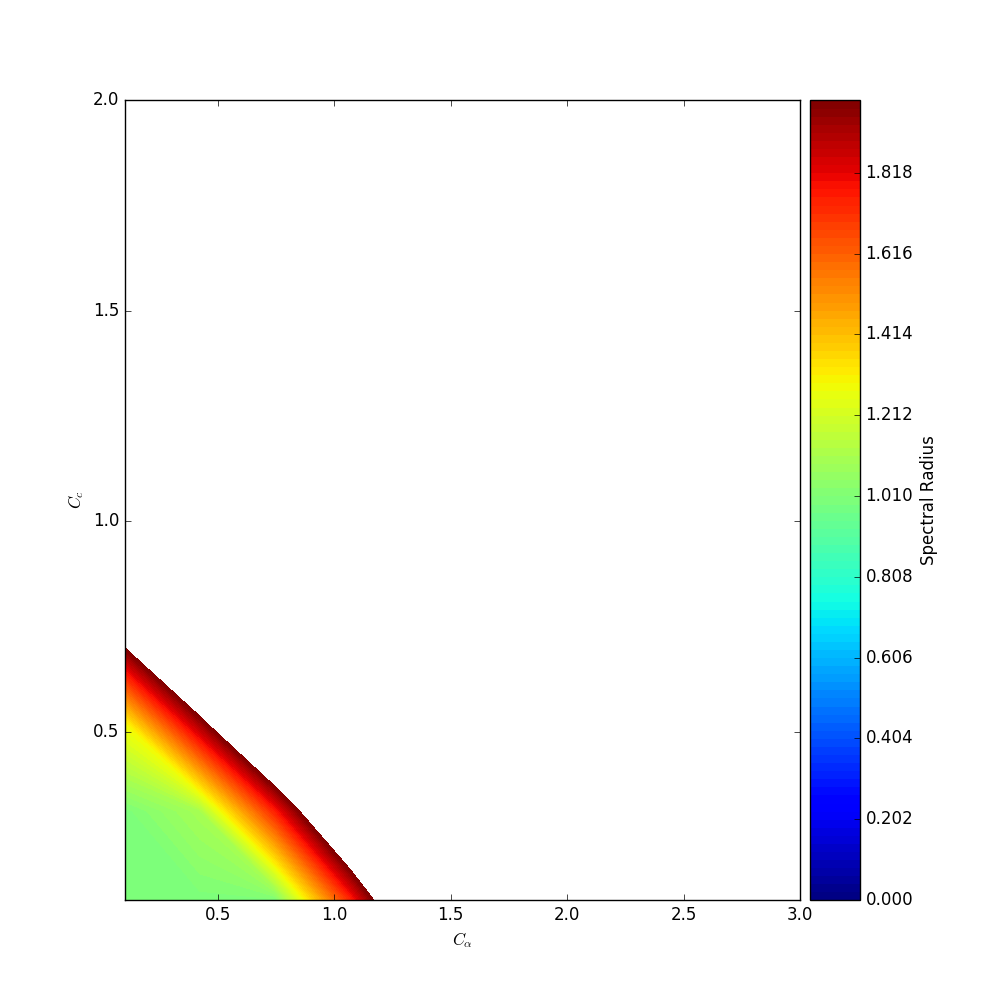
\includegraphics[scale=0.35]{p2e_contours_u1st.png}
 \caption{Flooded Iso-contour of Spectral Radius for 1st-order-upwind}
\label{label}
\end{figure}
\end{problem}

\begin{problem}{3}
\text{}\\
$(a)$ From Figure 19, we can see the evolution from transient states to steady state which is the line with Final Time label, we can see that the solutions $u(x,t)$ all converge into a point on $u=0$ at steady state, where that point can be defined as $\delta$ by $u(\delta) = 0.01a$.\\
For this original parameter combination, they are $L = 1$, $c=10$, $\alpha=2$, $\beta=10$, $\omega=100000$, $a=1$. And we can get that the $\delta = 0.5102$ by set a tolerance of $1 \times 10^{-6}$ and calculate the different between each $\delta$ for each transient state, and got the steady state when the $\delta$ difference is within the tolerance.\\
\begin{figure}[H]
\centering
  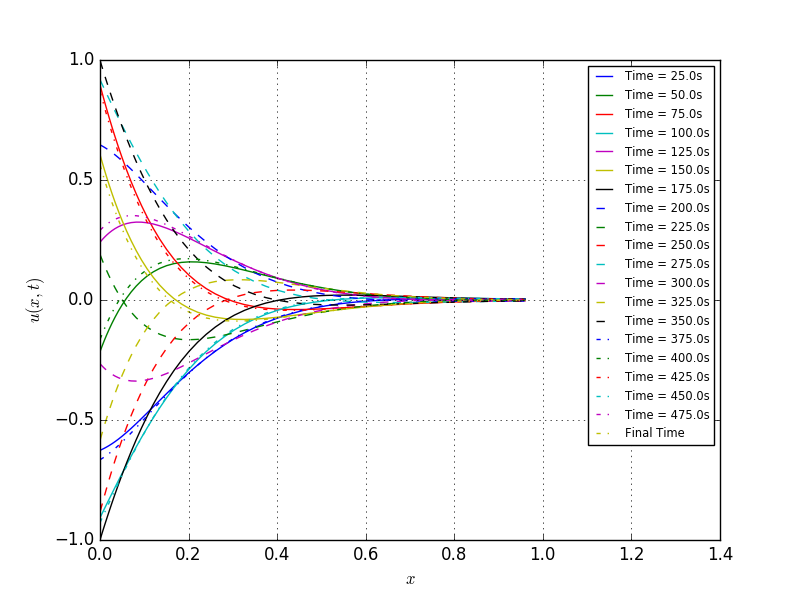
\includegraphics[scale=0.5]{p3a_ss.png}
 \caption{Transient and Steady State Solution}
\label{label}
\end{figure}
\text{}\\
$i)$ Change $c$ from 10 to 20 and 30. $c$ is the advection speed, so larger $c$ will cause larger convection, which means the solution is moving faster and has bigger amplitude(convection input).\\
\begin{figure}[H]
\centering
  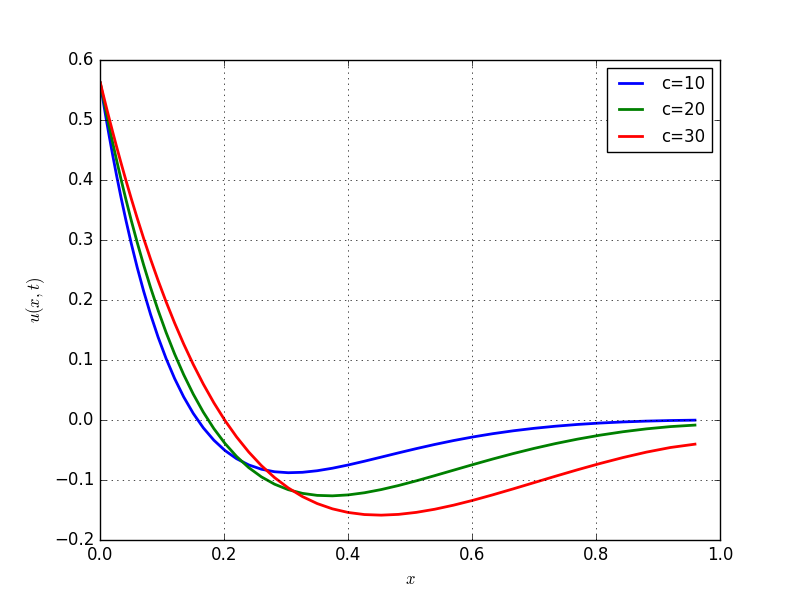
\includegraphics[scale=0.6]{p3a_change_c.png}
 \caption{Showcase of changing $c$}
\label{label}
\end{figure}
\text{}\\
$ii)$ Change $\alpha$ from 2 to 5 and 10. $\alpha$ is the diffusive coefficient, so larger $\alpha$ will cause more obvious diffusive phenomenon and smaller amplitude.\\
\begin{figure}[H]
\centering
  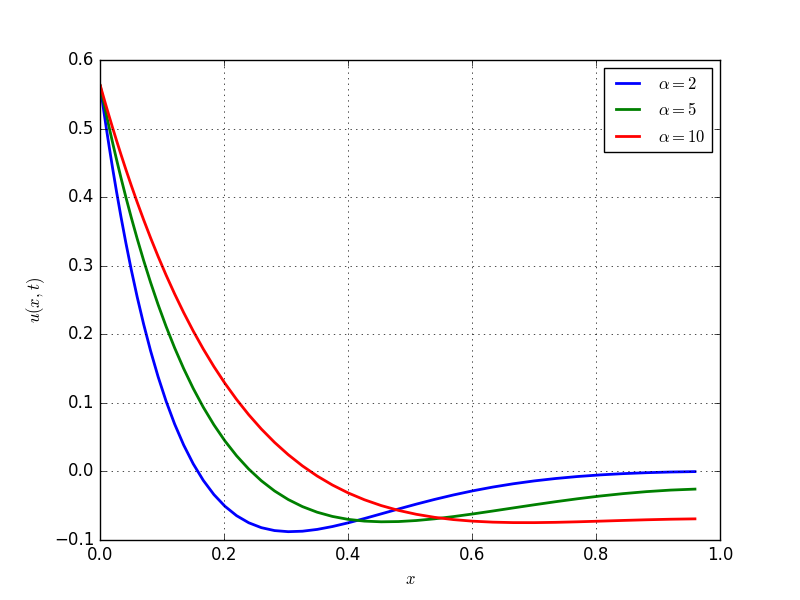
\includegraphics[scale=0.6]{p3a_change_alpha.png}
 \caption{Showcase of changing $\alpha$}
\label{label}
\end{figure}
\text{}\\
$iii)$ Change $\beta$ from 10 to 100 and 1000. $\beta$ is the damping coefficient. It controls how fast the curve reach the steady state, so larger $\beta$ will damp faster and have smaller $\delta$.\\
\begin{figure}[H]
\centering
  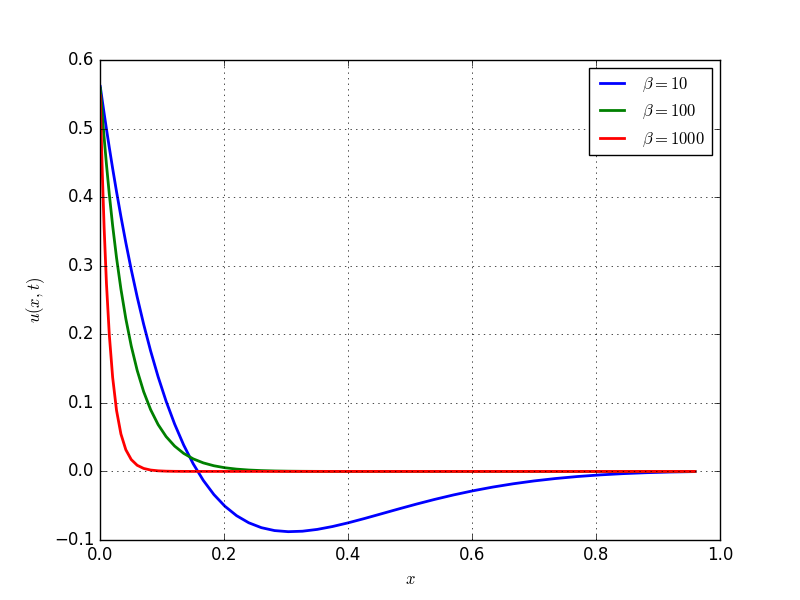
\includegraphics[scale=0.5]{p3a_change_beta.png}
 \caption{Showcase of changing $\beta$}
\label{label}
\end{figure}
\text{}\\
$iv)$ Change $\omega$ from 100000 to 10000 and 1000. $\omega$ is the angular frequency of the boundary condition. Larger  $\omega$ will have smaller period and larger frequency.\\
\begin{figure}[H]
\centering
  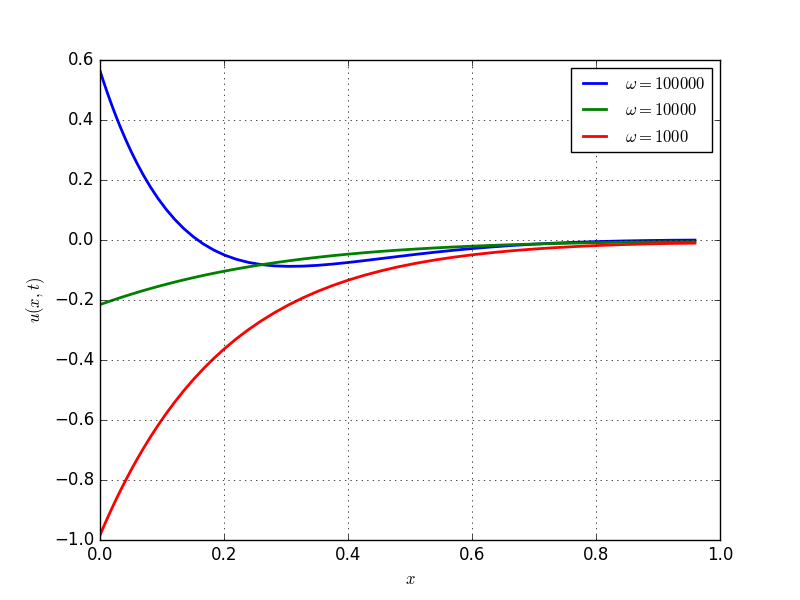
\includegraphics[scale=0.5]{p3a_change_w.png}
 \caption{Showcase of changing $\omega$}
\label{label}
\end{figure}
\text{}\\
$v)$ Change $a$ from 1 to 2 and 3. $a$ is the amplitude of the left bound boundary condition. It controls the upper and lower bounds of the solutions. As you can see, solutions are self-similar with bounds limited to $a$\\
\begin{figure}[H]
\centering
  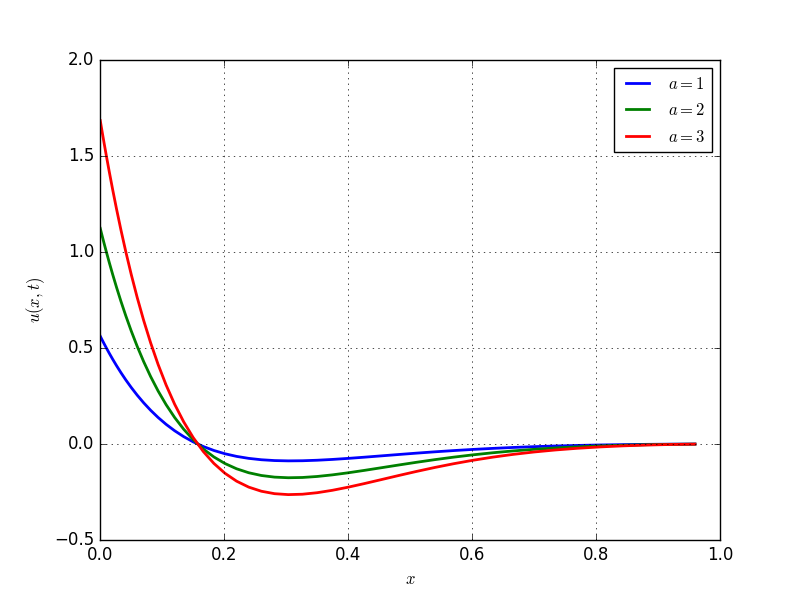
\includegraphics[scale=0.5]{p3a_change_a.png}
 \caption{Showcase of changing $a$}
\label{label}
\end{figure}
\text{}\\
$(b)$ By adopting $\Pi$ - theorem, we can get 5 $\Pi$ groups, where $num_{var} - num_{dim} = 7 - 2 = 5.$\\
\\
The two dimensions are $L$(length) and $T$(time).\\
\\
For the seven parameters, $\delta = [L]$, $c = [\frac{L}{T}]$, $\alpha = [\frac{L^2}{T}]$, $\beta = [\frac{1}{T}]$, $L= [L]$, $a = [\frac{L}{T}]$, $\omega = [\frac{1}{T}]$\\
\\
First, we want to eliminate $L= [L]$, so $\frac{\delta}{L} = [1]$(No dimension),  $\frac{c}{L} = [\frac{1}{T}]$,  $\frac{\alpha}{L^2} =  [\frac{1}{T}]$, $\beta = [\frac{1}{T}]$, $\frac{a}{L} =  [\frac{1}{T}]$, $\omega = [\frac{1}{T}]$.\\
\\
Then, we want to eliminate $\omega = [\frac{1}{T}]$, then $\frac{\delta}{L} = [1]$, $\frac{c}{L\omega} = [1]$, $\frac{\alpha}{L^2 \omega} = [1]$, $\frac{\beta}{\omega} = [1]$, $\frac{a}{L\omega} = [1].$\\
\\
So we can get: $\frac{\delta}{L} = f(\frac{c}{L\omega}, \frac{\alpha}{L^2 \omega}, \frac{\beta}{\omega}, \frac{a}{L\omega})$\\
\\
From Figure 25, we can see that by change $L$ linearly with slope of 2 and keep all other 4 $\Pi$ groups constant, we can get $\delta$ changing linearly with the same slope as $L$.\\
\begin{figure}[H]
\centering
  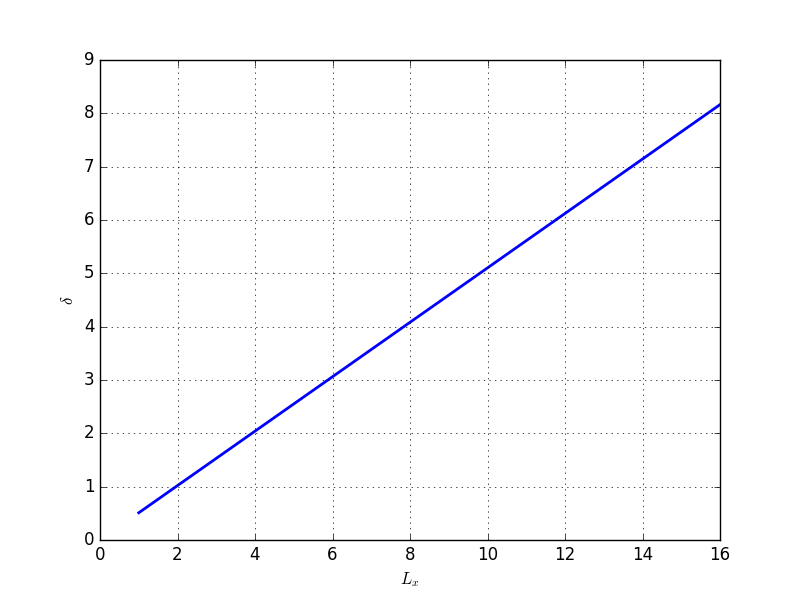
\includegraphics[scale=0.65]{p3b.png}
 \caption{Relationship between $\delta$ and \L with the other $\Pi$ groups constant}
\label{label}
\end{figure}

\end{problem}
\end{document}
